\documentclass{report}
\usepackage{graphicx}
\usepackage{listings}
\usepackage{xcolor}
\usepackage{array}
\usepackage[a4paper, total={6in, 10in}]{geometry}

\definecolor{codegreen}{rgb}{0,0.6,0}
\definecolor{codegray}{rgb}{0.5,0.5,0.5}
\definecolor{codepurple}{rgb}{0.58,0,0.82}
\definecolor{backcolour}{rgb}{0.95,0.95,0.92}

\lstdefinestyle{mystyle}{
	backgroundcolor=\color{backcolour},   
	commentstyle=\color{codegreen},
	keywordstyle=\color{magenta},
	numberstyle=\tiny\color{codegray},
	stringstyle=\color{codepurple},
	basicstyle=\ttfamily\footnotesize,
	breakatwhitespace=false,         
	breaklines=true,                 
	captionpos=b,                    
	keepspaces=true,                 
	numbers=left,                    
	numbersep=5pt,                  
	showspaces=false,                
	showstringspaces=false,
	showtabs=false,                  
	tabsize=2
}
\lstset{style=mystyle}
\graphicspath{ {images/} }
\title{Operating Systems\\ HoGent}
\author{JeeVeeVee}
\date{2020/2021}
\begin{document}
	\maketitle
   	\tableofcontents
   	\chapter{besturingssysteem}
	   	\section{Wat is een besturingssysteem}
		   	Een besturingssysteem is de link tussen hardware en de gebruiker.  Zonder besturingssysteem zou de gebruiker rechtstreeks de hardware moeten aanspreken, wat quasi onmogelijk is. 
		  	Een besturingssysteem is een programma dat het mogelijk maakt de hardware van een computer te gebruiken. Een afkorting die vaak wordt gebruikt is OS (Operating System)
		   	De taken van een OS zijn : 
		   	\begin{itemize}
		   		\item opslaan en ophalen van info 
		   		\item programma's afschermen 
		   		\item gegevenstroom regelen 
		   		\item prioriteiten regelen
		   		\item beheer en delen van bronnen 
		   		\item tijdelijke samenwerking tussen programma's mogelijk maken 
		   		\item reageren op fouten 
		   		\item tijdsplanning maken 
	  		\end{itemize}
	  	 	Voorbeelden van OS's zijn Windows, MacOS, linux distros,...
	  	 \section{Soorten besturingssystemen}
	  	 	We maken een onderscheid tussen : 
	  	 	\begin{itemize}
	  	 		\item single-tasking systemen 
	  	 		\item multi-tasking single user systemen 
	  	 		\item multi-user systemen 
	  	 	\end{itemize}	  	 	
  	 	\section{Concepten van besturingssystemen}
  	 		\subsection{verschillende lagen}
  	 			Veel OS's implementeren de interface tussen gebruiker en computer als een reeks stappen of lagen. In de toplaag zijn de functies vastgelegd en de onderste laag bevat de details van het laagste niveau om deze functies uit te voeren. De gebruiker communiceert altijd met de bovenste laag, deze laag noemen we de shell of de command interpreter. De shell geeft op zijn beurt de opdrachten door aan de laag onder hem. Uiteindelijk komt de opdracht (versnippert) aan bij de onderste laag : de kernel. De kernel is het hart van het OS. 
  	 		\subsection{programma's en taken}
  	 			Een OS zorgt ervoor dat taken uitgevoerd worden, we maken hierbij een onderscheid tussen : 
  	 			\begin{itemize}
  	 				\item interactieve programma's
  	 					\subitem een programma dat de gebruiker vanaf de terminal activeert, over het algemeen is dit een korte opdracht, er wordt vaak een \textbf{snelle respons} verwacht.
  	 				\item batch programma's
  	 					\subitem programma's die geen directe respons verwachten, de opdrachten worden opgeslaan in een file, en worden toegevoegd aan een batch queue.
  	 				\item real-time programma's
  	 					\subitem Er is spraken van een tijdsbeperking, vaak nog snellere respons dan bij interactieve programma's
  	 			\end{itemize}
   			\subsection{processen}
   				Een proces zijn 1 of meerdere opdrachten die door een programma worden beschouwd als 1 eenheid. Een programma of taak bestaat vaak uit 1 of meerdere processen. Elk proces is dus onafhankelijk en dingt mee naar het gebruik van bronnen. Een OS houdt zich vaak voornamelijk bezig met het uitvoeren van processen, het verdeelt de bronnen en bepaald de volgorde.
   			\subsection{resources}
   				In eerste instantie moet een proces resources aanspreken. Het OS moet dan : 
   				\begin{itemize}
   					\item zorgen voor voldoende geheugen voor het proces
   						\subitem Een proces moet zijn instructies en gegevens kunnen opslaan. Geheugen is echter eindig, en dus moet het OS het verdelen. 
   					\item het gebruik van de CPU regelen 
   						\subitem Er zijn gewoonlijk meer processen dan CPU's, en dus moet het OS het gebruik ervan regelen, dit gebeurt op basis van prioriteit.
   					\item de gegevensstroom regelen van of naar randapparatuur
   						\subitem bv printers waar meerdere mensen op willen printen
   					\item bestanden of records kunnen lokaliseren
   						\subitem het lokaliseren van files en records 
   				\end{itemize}
   			\subsection{Scheduling}
   				Bij multi-tasking, en in het bijzonder mulit-user systemen is scheduling heel erg belangerijk. Scheduling verwijst naar de manier waarop processen een prioriteit krijgen toegewezen, vaak in combo met een prioriteiten wachtrij, dit komt later nog aan bod.
   			\subsection{Concurrency}
   				Processen zijn vaak niet onafhankelijk, ze zijn dan concurrent. Dit wil zeggen dat 2 processen soms ook dezelfde resources aanspreken, dit zorgt voor conflicten. Het OS moet de volgorde van de processen zodanig regelen, dat die conflicten worden vermeden, dit noemt \textbf{syncronisatie}.
   	\chapter{Virtualisatie \& Cloud}
   		\section{Wat is virtialisatie?}
   			Virtualisatie verwijst naar het creëren van een virtuele versie van iets, zoals virtuele computer hardware, opslagapparaten, netwerkbronnenn,... Traditioneel gebruiken we 1 OS op een computer, dat OS spreekt de hardware aan, en de applicaties draaien er bovenop. Door middel van virtualisatie kan men op 1 computer meerdere (virtuele) computers laten draaien. Die virtuele computers delen van fysieke hardware.
   			\\
   			De voordelen van virtualisatie is dat het efficiënter gebruik maakt van de beschikbare ruimte, het is goedkoper en de ecologische voetafdruk verkleint eveneens. 
   			\\
   			Virtualisatie bestaat in veel vormen en maten. 1 van de bekendste spelers op de markt is VMware, maar ook grote bedrijven als Microsoft en Oracle mengen zich. Docker is een vrij nieuwe en speciale vorm van virtualisatie, er worden geen virtuele machines gebruikt, maar er wordt een linux kernel gebruikt door meerdere containers.
   		\section{Concepten van virtualisatie}
   			\subsection{Virtuele Machine}
   				Een virtuele machine (VM) is een computerprogramme dat een volledige pc nabootst, en waar andere programma's op kunnen worden uitgevoerd. Een VM bezit vRAM, vCPU en een virtual disk.
   			\subsection{Soorten VM's}
   				\begin{itemize}
   					\item Programmeertaal-specifiek : JVM
   					\item Emulator : VirtualBox, VMWare
   					\item Applicatie-Specifiek : Docker
   				\end{itemize}
   			\subsection{Hypervisor}
   				Een hypervisor is de software die gebruikt wordt om VM's aan te maken en op te starten, deze worden soms ook Virtual Machine Monitor genoemd (VMM). Deze regelt de virtualisatie, en door er van gebruik te maken, kan 1 host pc meerder VM's tegelijkertijd laten draaien. 
   				\begin{itemize}
   					\item Type 1
   						\subitem native hypervisor
   						\subitem er is geen onderliggend OS
   						\subitem kan de hardware rechtstreeks aanspreken
   						\subitem geen overhead door OS
   						\subitem efficient maar ook complex
   						\subitem handig voor servers
   					\item Type 2
   						\subitem programma bovenop OS (VMWare)
   						\subitem het aanspreken van hardware gebeurt via functies van het onderliggend OS
   						\subitem eenvoudig 
   						\subitem vooral gebruikt op persoonlijke toestellen 
   						\subitem niet zo krachtig
   				\end{itemize}
   		\section{Multi-tenacy}
   			Multi-tenacy is een concept dat veel ouder is dan computers, het stamt uit de immo markt. Een single tenacy is als er maar 1 huurder in een gebouw woont, zoals in een alleenstaande woning. Een appartement is multi-tenacy omdat het meerdere gezinnen kan huisvesten. De link met IT is dat een persoonlijke computer alleen door jou wordt gebruik, terwijl een fysieke server in een datacenter gedeeld wordt met veel klanten. 
   			\\ kenmerken : 
   			\begin{itemize}
   				\item bronnen worden gedeeld
   				\item een huurder is een gebruiker of een groep van gebruikers met gemeenschappelijke toegang 
   				\item er zijn verschillende vormen, zowel op niveau van hard als software
   				\item virtualisatie speelt een belangerijke rol
   				\item multitenacy is belangerijk kenmerk van Cloud Computing
   			\end{itemize}
	   		\begin{center}
	   			\begin{tabular}{| m{20em} | m{20em} | }
	   				\hline
	   				\textbf{voordelen} & \textbf{nadelen} \\
	   				\hline
	   				
					Efficienter gebruik van de beschikbare bronnen, er kunnen immers meerdere eindgebruikers door 1 toestel worden bediend
	   				 & Minder isolatie en verhoogde beveiligingsrisico's : 1 inbreuk op 1 instantie kan andere tenants treffen \\ 
	   				\hline
	   				lagere operationele kosten, en dus goedkoper voor de eindgebruiker & minder prestatie-isolatie, grote tenants kunnen de presatie van kleinere tenants negatief beïnvloeden \\  
	   				\hline
	   			\end{tabular}
	   		\end{center}
   		\section{Cloud Computing}
   			Bij Cloud computing worden computerbronnen, zoals hardware, software en gegevens, op aanvraag beschikbaar gesteld via een netwerk (meestal internet). De term is afkomstig uit de schematechnieken uit de informatica.
   			\\
   			kenmerken : 
   			\begin{itemize}
   				\item bronnen beschikbaar op aanvraag, vaak zonder tussenkomst van een fysieke persoon
   				\item vaak via een pay-as-you-go pricing model 
   				\item elasticiteit : mogelijk om automatisch aan te passen in functie van de vraag. 
   			\end{itemize}
   			\subsection{Cloud}
   				De cloud is een wolk van computers, een virtualisatie van de serveromgeving. De eindgebruiker weet niet waar de instanties precies draaien, en weet ook niet op hoeveel servers. Daardoor is de eindgebruiker geen eigenaar van hard/software, en is hij niet verantwoordelijk voor onderhoud. De cloud is een virtuele en schaalbare infrastructuur. 
   			\subsection{Deployment modellen}
   				\begin{itemize}
   					\item \textbf{Publieke} Cloud omgeving : beschikbaar voor iedereen, via het internet
   					\item \textbf{Private} Cloud omgeving : beperkte toegang tot 1 of meerdere organisaties, kan zelf in privaat of publiek datacenter.
   					\item \textbf{Hybride} Cloud omgeving : combinatie van meerdere modellen.
   				\end{itemize}
   			\subsection{Service modellen (publieke cloud)}
   				\begin{itemize}
   					\item \textbf{infrastructure} as a Service (laaS) : de infrastructuur wordt beschikbaar voor de gebruiker, die controle heeft over het OS, de software en de (virtuele) hardware. 
   					\item \textbf{Platform} as a Service (paaS) : platform en diensten worden aangeboden, de gebruiker heeft controle over de software, maar niet over de hardware.
   					\item \textbf{software} as a Service (saaS) : het aanbieden van louter software zoals office 365 
   				\end{itemize}
   				\begin{center}
   					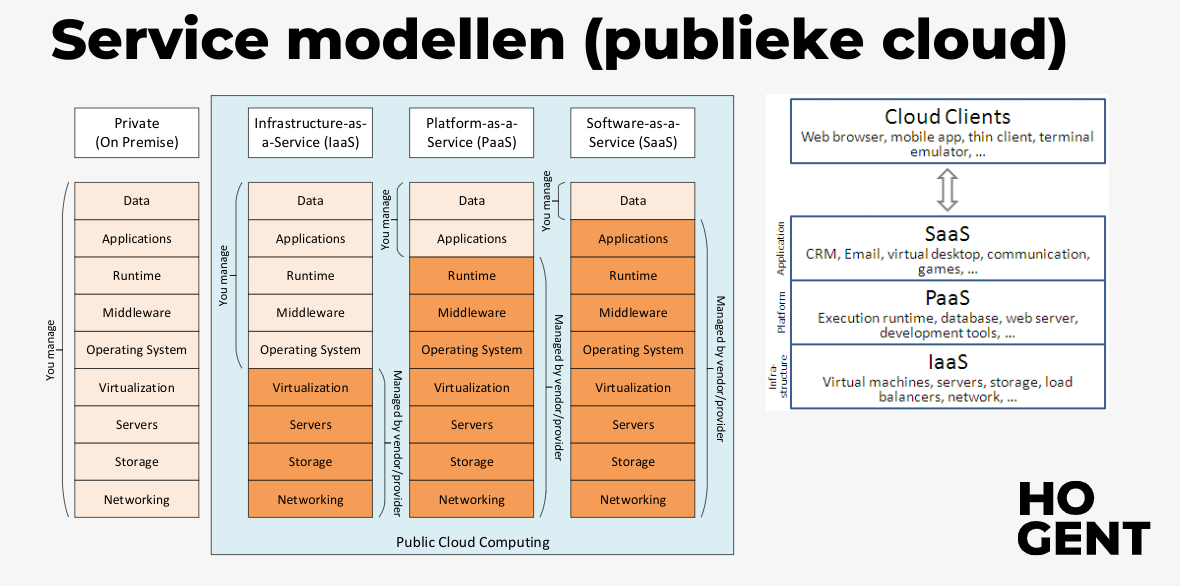
\includegraphics[scale=0.4]{service_modellen}
   				\end{center}
   			Virtualisatie speelt een belangerijke rol binnne Cloud Computing, er worden namelijk vaak virtuele bronnen beschikbaar gesteld aan de eindgebruiker. Zonder gebruik te maken van virtualisatie zouden er veel minder klanten gebruik kunnen maken van de Cloud omgeving en zouden er veel bronnen verspild worden. 
   			\subsection{Elasticiteit van de Cloud}
   				Het aanbod kan zich afstellen op de vraag, waardoor bv op piekmomenten meer bronnen beschikbaar zijn dan op andere momenten. Cloud Computing is een goed voorbeel van multi-tenacy.
   	\chapter{Processen}
   		\section{van programma tot proces}
   			Een programma dat geschreven is in een programmeertaal is niet meteen uitvoerbaar door de hardware, de CPU verstaat geen Java, C, C\#,... Elk programma moet dus tot een verzameling van instructies uit de instructieset van de CPU, dit proces noemt \textbf{compileren}. De code wordt dan eerst omgezet naar assambler taal, die op zijn beurt wordt omgezet naar binare code. de instructieset verschilt tussen types CPU, en het programma moet dus voor elk type CPU appart worden gecompileert.
   			\subsection{instructiecyclus}
   				Computerhardware werkt steeds op een oneindig lange cyclus, het bestaat uit 2 stappen : Fetch en Execute.
   				Een CPU maakt gebruik van verschillende registers voor het uitvoeren van de cyclus : 
   				\begin{itemize}
   					\item PC (program counter) houdt het adres bij van de uit te voeren instructie
   					\item IR (instruction register) : houdt de uit te voeren instructie bij
   					\item  AC (ACumulator) : hulpregister voor opslaan van tussenresultaten
   				\end{itemize}
   			\subsection{interuption}
   				Er kan altijd iets fout gaan waardoor een proces wordt stopgezet, de pc reageert hier op door een een proces te onderbreken, de fetch-execute loop wordt dan uitgebreid zodat dit mogelijk is? 
   			\subsection{binaries}
   				Het bestand dat wordt gegenereerd door het compilatieproces wordt een binary of een executable genoemd. Deze zijn afhankelijk van het besturingssysteem, wat er voor zorgt dat programmeurs ook voor elk verschillend besturingssysteem een apparte binary voorzien. 
   				\\
   				Eenmaal de binary is aangemaakt kan deze worden opgeslaan op de harde schijf, als de gebruiker dan dit programma wil uitvoeren, worden de instructies gekopieerd naar het RAM geheugen. De instantie van het programme in het RAM geheugen wordt een \textbf{proces} genoemd. Dan verandert het programma namelijk van iets passiefs naar iets actiefs. 
   		\section{opbouw van een proces}
   			Een \textbf{proces} is een instantie van een programma dat uitgevoerd wordt op het systeem. Ze zijn een belangerijk onderdeel van besturingsystemen. Een proces kan je zien als een soort container die alles bevat om een programma uit te voeren. Een proces is ook de reden dat meerdere programma's tegelijkertijd kunnen worden uitgevoerd. 
   			\subsection{proces image}
   				Een proces image is hoe een proces er uit ziet in het RAM geheugen, het bestaat uit : 
   				\begin{itemize}
   					\item text : de uit te voeren instructies 
   					\item data : globale variabelen 
   					\item stack : tijdelijke opslag voor variabelen, functieparameters, adressen,...
   					\item heap : dynamisch gealloceerd geheugen. 
   				\end{itemize}
   			\subsection{Proces Control Block}
   				Het OS heeft een overzicht van alle processen die acief zijn op het systeem. Dit overzicht heeft de vorm van een tabel en wordt ook wel de proces table genoemd. Een element uit zo een proces noemen we een \textbf{Proces Control Block}, die bevat volgende info : 
   				\begin{itemize}
   					\item info om het proces uniek te identificeren (id)
   					\item info om de staat van het proces bij te houden
   					\item info om het proces te beheren
				\end{itemize}   
		\section{soorten procesen}
			\subsection{interactief proces}
				Kan je zowel opstarten als controleren vanuit een terminal sessie, kunnen zowel in de voor- als op de achtergrond draaien. 
			\subsection{Automatisch proces}
				Worden ook wel batch processen genoemd, omdat er vaak meerdere zijn. Staan in een wachtrij, bij uitvoering worden alle processen uit de wachtrij 1 voor 1 uitgevoerd, en dit volgens het FIFO principe. 
			\subsection{daemons}
				Dit zijn processen die continu draaien, worden meestal gestart bij het opstarten van het systeem. Ook gekend als services.
		\section{beheer van processen}
			Het onstaan van een proces is verschillend in elk OS, hier behandelen we linux. In Linux heeft elk proces een eigen ID, de Proces IDentifier (PID). Het eerste proces dat wordt gecreëerd is steevast het opstarten van het systeem, en dit proces heeft dan ook altijd PID 1. Dit PID1 is het moederproces voor alle andere processen. Het aanmaken van een proces in linux bestaat ui het aanroepen van 2 functies : forkk() en exec(). Fork() maakt een exacte kopie van het proces in het RAM geheugen en vult de PID van het proces in, daarnaast worden ook de PPID (Parent PID). De exec() vult het nieuwe kindproces met de nodige waarden en instructies. Het einde van het proces maakt gebruik van de functie exit(), als er iets fout gaat kan er dan sprake zijn van orphan processes, processen die geen ouder meer hebben. De output van de exit() functie geeft aan of er iets fout is gegaan bij het uitvoeren, dan is de output \(\neq\) 0
			\pagebreak
   			\subsection{2|5|6 states}
   				Over het algemeen hebben processen altijd 1 van 2 states, running of not running. We zouden dit echter kunnen uitbreiden naar 5 states: 
   				\begin{itemize}
   					\item \textbf{new} : een nieuw proces werd aangemaakt door het OS, meestal is de PCB al toegevoegd aan de process table, maar nog niet volledig geladen in het geheugen. Als er een limiet wordt gezet op het aantal processen in de wachtrij, dan kan het proces nog niet overgaan van new naar ready.
   					\item \textbf{ready} : proces in de queue, klaar om uitgevoerd te worden door CPU
   					\item \textbf{running} : het proces wordt uitgevoerd door CPU
   					\item \textbf{blocked} : een proces staat te wachten op iets 
   					\item \textbf{exit} : afgewerkt proces, niet perse goed afgewerkt!!
   				\end{itemize}
   				We zouden zelfs een \(6^{de}\) state kunnen toevoegen: \textbf{suspend}, dit komt voor wanneer er te weinig geheugen is, dit kan worden opgelost door data weg te schrijven naar de harde schijf. Dit proces noemt swapping, dit is een vrij intensief proces, maar als het niet gebeurt dan crasht het systeem. 
   				\begin{center}
   					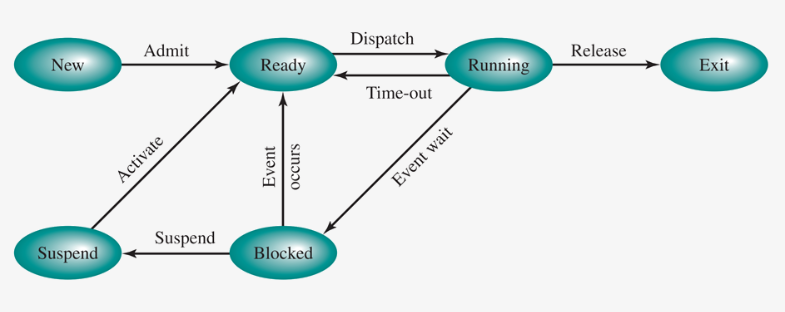
\includegraphics[scale=0.6]{six_states}
   				\end{center}
   		\section{Scheduling}
   			Een OS zal steeds proberen om de hardware zo optimaal mogelijk te gebruiken, dit wil zeggen dat het zal vermijden dat een deel van de CPU niet aan het werken is. Het is echter wel belangerijk dat de CPU Utilisation niet 100\% wordt, want dan kan de CPU geen interrupts meer verwerken! Het niet verloren laten gaan van CPU-tijd noemt men \textbf{multi-programming}	
   			\subsection{time sharing}
   				Time sharing is het OS dat processen kort laat afwisselen op de CPU zodat het voor de gebruiker lijkt alsof de 2 processen simultaan runnen. 
   			\subsection{context switch}
   				Bij het wisselen van een proces (bv bij time sharing) treedt er een \textbf{context switch op}: er wordt een \textbf{snapshot} genomen van het volledige proces en wordt bewaard in het geheugen, dan wordt er een snapshot van het ander proces ingeladen en wordt dat proces uitgevoerd.
   			\subsection{Scheduler}
   				De \textbf{scheduler} is verantwoordleijk voor het bepalen wanneer welk proces CPU tijd krijgt. Hij houdt daarbij rekening met : batch, interactive, realt ime. Het zijn dan ook complexe systemen. Er bestaan meedere verschillende algoritmes voor schedulers, we kunnen ze algemeen verdelen in : 
   				\begin{enumerate}
   					\item \textbf{non-preemptive} : algoritmes die geen gebruik maken van context switches en dus pas wisselen van proces wanneer een proces volledig is afgewerkt.
   					\item \textbf{preemtive} : er wordt gebruik gemaakt van context switches.
   				\end{enumerate}
   				Enkele voorbeelden : 
   				\begin{itemize}
   					\item \textbf{First Come First Serve (FCFS)} : een non-preemptive algrotime dat gebruikt maak van een eenvoudig wachtrij, nieuwe processen schuiven achteraan aan. Er kan geen starvation optreden maar het zou kunnen dat korte processen lang moeten wachten.
   					\item \textbf{Shortest Proces Next (SPN)} : een non-preemptive algoritme waarbij er gebruik wordt gemaakt van een eenvoudige wachtrij, elk proces wordt volledig afgewerkt, waarna het de beurt aan het volgende proces dat de korste uitvoeringstijd heeft op de wachtij. Korte processen kunnen snel worden uitgevoerd maar er is risico op starvation voor lange processen.
   					\item \textbf{Shortest Remaining Time (SRT)} : een preemptive algoritme dat op dezelfde manier werkt als SPN. De korte processen worden snel uitgevoerd maar ook hier is er risico op starvation voor lange processen, bovendien is er ook de overheid bij veel wissels
   					\item \textbf{Round Robin (RR)} : preemtive waarbij de CPU na Q eenheden wisselt naar het volgend proces in de rij, het huidige proces wordt dan achteraan de rij toegevoegd als het nog niet klaar was. Dit is heel eerlijk, maar de waarden van Q is heel belangerijk, korte processen lopen het risico lang te moeten wachten en er is de overhead door het wisselen. 
   				\end{itemize}
   	\chapter{Concurrency}
   		\section{Wat is concurrency}
   			We kunnen een onderscheid maken tussen : 
   			\begin{itemize}
   				\item \textbf{multiprogramming} : het beheer van meerdere processen met 1 processor
   				\item \textbf{multiprocessing} : het beheer van meerdere processen met meerdere pcoressoren.
   				\item \textbf{gedistrubeerde verwerking} : het beheel van meerdere processen die worden uitgevoerd op meerdere computersystemen.
   			\end{itemize}
   			Een \textbf{multiprocessor} is een systeem met \(>\) 1 CPU's, dergelijke systemen kunnen meerdere systemen gelijktijdig uitvoeren, dit noemen we \textbf{concurrency}. Concurrency verhoogt de producticitiveit, maar zorgt ook voor uitdagingen. \\
   			Concurrency kan optreden in meerdere situaties, ook bij systemen met maar 1 CPU: 
   			\begin{itemize}
   				\item meerdere toepassingen : er zijn verschillende processen gelijktijdig actief, er wordt gebruik gemaak van multiprogramming om de processortijd dynamisch te verdelen over het aantal actieve toepassingen. 
   				\item gestructureerde toepassingen : Als uitbeiding op de beginselen van modulair ontwerpen en gestructureerd programmeren kunnen sommige toepassingen zondag zijn geprogrammeerd asl een verzameling van een aanal actieve toepassingen (multi-threading)
   				\item structuur van OS : OS's zelf worden vaak geïmplementeerd als een verzameling processen. 
   			\end{itemize}
   			\subsection{paralellism}
   				De term \textbf{parallelism} betekent dat een toepassing zijn werk opsplitst in meerder subtaken die parallel kunnen worden verwerkt.
   		\section{Wederzijdse uitsluiting (mutual exclusion)}
   			Soms, als bronnen worden gedeeld over meerdere processen, dan kan het gebeuren dat meerdere processen tegelijktijd dezelfde bron willen aanspreken. Het deel van het proces dat een (gedeelde) bron aanspreekt noemen we de \textbf{kritieke sectie}. Het is belangerijk dat altijd slechts 1 proces in de kritieke sectie zit. \textbf{Wederzijdse uitsluiting} is een term die aanduid dat een 2 processen op elkaar wachten om een gedeelde bron aan te spreken. Het is niet evident om wederzijdse uitsluiting af te dwingen, je kan gebruik maken van algoritmes of andere alternatieven. 
   		\section{Syncronisatie}
   			\textbf{Synchronisatie} is het proces of het resultaat van iets gelijktijdig maken, in deze context is dat het opleggen van een dwingende volgorde aan events, die door concurrente asynchrone processen worden uitgevoerd. Je moet hierbij garanderen dat processen in een bepaalde volgorde verlopen. 
   			\subsection{bestandssynchronisatie}
   				\textbf{Bestandssynchronisatie} is een voorbeel van synchronisatie waarbij 2 of meerdere bestanden aan elkaar gelijkgesteld worden. De inhoud van deze bestanden zal dan op 2 of meerdere plekken hetzelfde zijn. (kopie) 
   		\section{Deadlocks}
   			Een \textbf{deadlock} is een situatie waarbij een bepaalde actie is vastgelopen op wederzijdse uitsluiting. Meerdere processen zitten tegelijkertijd in de kritieke sectie. Irl kan je ze vergelijken met overbevolkte kruispunten waar na verloop van tijd iedereen vaststaat. Je kan omgaan met deadlocks door ze te voorkomen of door ze te detecteren en herstellen. Deadlocks kunnen enkel optreden bij : 
   			\begin{itemize}
   				\item bron met wederzijdse uitsluiting
   				\item proces zal bron bezet houden en wachten 
   				\item er is geen voortijding ontemen 
   				\item processen wachten in een kring
   			\end{itemize}
   			\subsection{Deadlock preventie}
   				Basically, zrog ervoor dat der voorwaarden voor een deadlock nooit optreedt. Sommige voorwaarden zijn echter noodzakelijk, en er ontstaan nog grotere problemen als je ze opheft. Vermijden \(>\) voorkomen. Als je de mogelijkheid voor deadlocks gwn heel klein maakt, is dit vaak genoeg. Op die manier blijft de omgeving veilig. 
   			\subsection{Deadlock signaliseren}
   				Er bestaan algoritmes om cycles in een graaf te vinden. daarna kan je (zie volgende titel xoxo)
   			\subsection{Deadlock herstellen}
   				1 van de processen moet worden stopgezet via KILL, je geeft dus de bron vrij ten koste van een proces, vervolgens vindt er een rollback plaats op het proces, zodat die alsnog wordt uitgevoerd. 
   	\chapter{File Systems}
   		\section{Persistente Opslag}
   			Processen maak gebruik van persistentie bijvoorbeeld wanneer ze data bewaren na het afsluiten van een proces, of als ze data willen delen met andere processen. Zoals je weet halen processen de data en de instructies die ze nodig hebben uit het RAM geheugen. RAM is echter beperkt in capaciteit. 
   			\subsection{Hard Disk Drive (HDD)}
   				Een HDD is een magnetisch opslagmedium dat een grote opslagcapaciteit biedt voor een lage prijs. Een HDD werkt met draaiende schijven, daardoor is er telkens een kleine vertraging \textbf{seek time} wanneer de leeskop zich beweegt naar de gevraagde data.
   			\subsection{Solid State Drive (SSD)}
   				Een SSD is sneller maar duurder dan een HDD. Het heeft geen draaiende onderdelen, maar maakt gebruik van circuits (IC's), waardoor de schijf robuuster is en geen seek time nodig heeft. 
   			\subsection{CD/DVD}
   				CD's en DVD's zijn optische opslagmedia, ze zijn beperkt in performantie en vaak read-only. Ze worden dan ook vaker gebruikt als distributiemedia of back-ups. 
   			\subsection{USB stick}
   				Deze maken ook gebruik van IC's, ze zijn echter externe opslagmedia dei worden aangesloten, hierdoor hebben ze beperkte capaciteit en performantie. 
   		\section{Files}
   			Een fysiek opslagmedium is onderverdeeld in blokken, een \textbf{file} (bestand) groepeert data  uit 1 of meerdere blokken. Het is dus een abstracte eenheid die de complexiteit van de fysieke opslag verbergt. De implementatie van files gebeurt door een \textbf{file system}. De gebruiker krijgt de file te zien als een opeenvolging van bytes, dit is dus een abstractie, in realiteit zijn die bytes verspreid over verschillende blokken die niet noodzakelijk aansluiten?
   			Een file heeft : 
   			\begin{itemize}
   				\item een naam, eventueel gevolgd door een extentie
   				\item een huidige en een maximale grootte 
   				\item toegangsrechten 
   				\item een datum van aanmaak en van laatste aanpassing 
   				\item een verwijzing naar de blokken waar de bytes van het bestand zijn opgeslagen. 
   			\end{itemize}
   		
	   		Binnen UNIX geld de regel \textit{"Everything is a file"}, dit houdt in dat zowel directories, links, speciale bestanden, sockets en pipes worden gezien als een file. \\
	   		Je kan bytes uitlezen op 2 verschillende manieren : 
	   		\begin{itemize}
	   			\item \textbf{sequentieel}, dan worden de bytes in volgorde uitgelezen, wat inhoud dat al je byte 100 wil lezen je dus ook bytes 1 - 99 moet lezen.
	   			\item \textbf{Random Access}, dan worden de bytes uitgelezen in willekeurige volgorde, wat inhoud dat je meteen naar byte 100 kan gaan als je dat zou willen. 
	   		\end{itemize}
   		\section{Directories}
   			Een directory groepeert bestanden, en andere directories, het creërt hierdoor een hiërarchische structuur. De implementatie gebeurt door het file system, elke file heeft dan zowel een absoluut (vertrekkende vanaf de root), en een relatief (vertrekkende vanuit de huidige locatie) pad. 
   		\section{File systems}
   			Een \textbf{file system} (bestandssystem) is een onderdeel van het besturingssysteem, ze beheren de fysieke opslagruimte en implementeren files en directories. Het is mogelijk voor een besturingssysteem om meerdere file system (tegelijk) te ondersteunen. 
   			\\
   			Er zijn verschillende implementaties voor files: 
   			\begin{itemize}
   				\item \textbf{Contiguous storage}, hierbij wordt elk bestand in 1 of meerdere aansluitende blokken opgeslagen. Deze eenvoudige methode geeft een goede leessnelheid en ondersteunt random access. De nadelen echter zijn dat als een bestand groeit, dat het eventueel moet worden verplaatst. en dat als een bestand wordt verwijderd, de vrije ruimte wordt ingenomen door een kleiner bestand waardoor er \textbf{fragmentatie} ontstaat. We vinden deze implementatie vaak terug op CD's en DVD's. 
   				\item  \textbf{linked lists}, hierbij hoeven de datablokken van een bestaand bestand niet aan te sluiten, aangezien elke blok een verwijzing bijhoudt naar het volgende blok. Hierdoor is er geen risico op fragmentatie, maar dat gaat ten koste van een goede performantie. Er is ook geen ondersteuning voor random access. 
   				\item \textbf{File Allocation Table (FAT)}, dit is een verbetering van de linked list techniek. De datablokken vormen nog steeds een linked list, maar alle verwijzingen tussen de blokken worden samengebracht in 1 tabel. Door deze tabel te bewaren in het RAM, verhoog je de leessnelheid en maak je random access mogelijk. Het nadeel hier is dat je een hoog RAM-verbruik kan hebben.
   				\item \textbf{index nodes (inodes)}, een inode is een datastructuur die zowel de metadata van een bestand als verwijzingen naar de datablokken bevat. Een bestandssysteem dat inodes gebruikt hoeft enkel de inodes van de geopende bestanden in het RAM te bewaren. Hierdoor kan deze techniek een goede leesbaarheid combineren met een beperkt RAM-verbruik. 
   			\end{itemize}
   			Ook de directories kan worden opgeslaan als een file, die file heeft dan 1 entry per subdirectory of file.
   			\\
   			Meeste file systems ondersteunen ook links, een link verwijst naar een ander bestand, ze bestaan in 2 vormen : 
   			\begin{enumerate}
   				\item een \textbf{hardlink} waarbij de datablokken / inodes worden gedeeld
   				\item een \textbf{soft link} waarbij de link een eigen datablok of inode heeft. 
   			\end{enumerate}
   			\subsection{Virtual file systems (VFS)}
   				Op windows krijgt elk bestandssysteem een drive letter(C, D), linux en mac hebben een virtual file system, dat alle bestandssystemen presenteert als 1 hiërarchische structuur. De processen maken dan gebruik van de algemene functies van het OS om het virtual file system aan te spreken, deze functies zijn dus NIET gebonden aan een specifiek file system. Het virtual file system vertaalt vervolgens deze algemene functieoproepen naar specifieke voor elk file systeem. Het inladen van een bestandssysteem binnen de VFS-hiërarchie heet een \textbf{mount} bewerking. Het uitladen is logischerwijs \textbf{unmount}.
   		\section{Partities}
   			Een fysiek opslagmedium kan zijn capaciteit onderverdelen in partities, elke partitie heeft zijn eigen bestandssysteem. Het opslagmedium voorziet een partitietabel die info bevat over de partities en hun bestandssysteem.
   			\\
   			\textbf{windows file systems : }
   			\begin{itemize}
   				\item NFTS : New Technology File System, maakt gebruik van journaling
   				\item FAT32 : File Allocation Table, gebruikt 32-bit addressering
   				\item exFAT : extensible File Allocation Table, gericht op USB en SD-kaarten, maakt gebruik van file allocation table, maar geen journaling
   			\end{itemize}
   			\textbf{mac: }
   			\begin{itemize}
   				\item HFS+ : Hierarchical File System +, gebruikt journaling, is verouderd
   				\item ADFS : Apple File System, focus op SSD en encryptie
   			\end{itemize}
   			\textbf{linux : }
   			\begin{itemize}
   				\item ext4 : fourth extended file system, gebruitk journaling
   				\item ZFS : zettabyte file system, heeeeeel geavanceerd
   				\item Btrfs : Better File system, antwoord op ZFS van oracle, op fedora
   			\end{itemize}
   			\textbf{andere :}
   			\begin{itemize}
   				\item ISO 9660 /UDF : voor optische schijven, gericht op write once-media
   			\end{itemize}
   	\chapter{Threads}
   		\section{Wat zijn threads}
   			Tot nu waren processen altijd atomair, het kon verschillende toestanden hebben via de scheduler, en toegang vragen tot rekenkracht of bestanden. We kunnen een proces echter opsplitsen in 2 concepten : 
   			\begin{itemize}
   				\item \textbf{Eigendom van bronnen} : het besturingssysteem dat er voor zorgt dat de processen elkaar bronnen niet zomaar beïnvloeden
   				\item \textbf{uitvoeren van instructies} : hiervoor wordt gebruik gemaakt van de Program Counter om de volgende instructie uit te voeren, en info bij te houden
   			\end{itemize}
   			Deze concepten staan eigenlijk los van elkaar
   			\subsection{proces : eigendom bronnen}
   				Elk proces krijgt controler of eigenaarschap over bronnen (locking). Hierdoor worden de bronnen afgeschermd door andere processen. Het uitvoeren van een proces volgt de fetch-execute cyclus voor het uitvoeren van de instructies.\\
   			\subsection{ threads}
   				Het Verschil tussen processen en threads, is dat een thread het uitvoeringsgedeelte van een proces is en dus niet op zichzelf kan bestaan. Binnen een proces kunnen er meerdere threads tegelijkertijd bestaan, die processen zijn dan \textbf{multi-threaded}. Een Thread bestaat uit : 
   				\begin{itemize}
   					\item thread ID
   					\item registers
   					\item stack 
   					\item toestand
   				\end{itemize}
				Threads binnen hetzelfde proces, delen de instructies, data en toegang tot bronnen. 
		\section{Soorten Threads}
   			\subsection{User-Level Threads}
   				Het OS beschouwt het programma als single-threaded proces, maar het programma maakt gebruik van een bibliotheek voor threading. De voordelen zijn dan de er geen system calls nodig zijn van het OS voor de threading (waardoor het sneller is), het proces heeft zelf geen controle over de scheduling threads, en je bent onafhankelijk van het OS (JVM). De nadelen echter zijn dat als de thread blokkeert op I/O, het hele proces wordt geblokkeerd, en er is geen gebruik van multiprocessing. 
   			\subsection{Kernel-Level Threads}
   				De logica voor deze threads zit in het OS, de voordelen hiervan zijn dat scheduling mogelijk is op threadniveau, dat het blokkeren van 1 thread geen invloed heeft op andere threads, mulitprocessing mogelijk is en dat het OS zelf ook threads gebruikt. Het nadeel is dat het trager is. 
   		\section{voor en nadelen}
   			\subsection{voordelen van multithreading}
   				\begin{itemize}
   					\item niet noodzakelijk om het hele proces te blokkeren 
   					\item eenvoudiger om bronnen te dleen 
   					\item lichter en sneller dan processen 
   					\item efficient gebruik van multi-core CPU's (parallellisme)
   				\end{itemize}
   			\subsection{uitdaingen bij multithreading}
   				\begin{itemize}
   					\item indelen van het rekenwerk in mogelijke threads
   					\item opsplitsen van data over de threads
   					\item afhankelijkheid van de data tussen threads
   					\item testen en debuggen
   				\end{itemize}
   		\section{Parallellisme}
   			\subsection{Soorten parallellisme}
   				Bij Parallellisme gaan we taken opsplitsen in verschillende subtaken, die onafhankelijk van elkaar uitgevoerd worden. Dit kan op verschillende manieren
   				\subsubsection{data parallellisme}
   					De te verwerken data wordt opgesplitst in stukken, op elk stuk wordt vervolgens dezeldfe ebwerking uitgevoerd. 
   				\subsubsection{taken parallellisme}
   					Taken parallellims verdeelt het werk op in verschillende threads, niet elke thread voert dezelfde operatie uit. 
   		\section{Amdahl's law}
   			De Wet van Amdahl is een manier op een theoretische schattin te maken hoe het toeveogen van cpu cores de uitvoering van een programma versneld. 
   			\[snelheidswinst = \frac{1}{S + \frac{1 - S}{N}}\]
   			Hierbij staat S voor het percentage van het programma dat sws ni versneld kan worden door meer CPU cores (als kommagetal) en N voor het aantal CPU cores
   			
\end{document}